\documentclass[english,10pt,a4paper]{article}

\usepackage{geometry}
\geometry{top=3cm, bottom=3cm, left=3cm , right=3cm}

\usepackage[utf8x]{inputenc}
\usepackage[french]{babel}
\usepackage{hyperref}

\usepackage{amsmath,amssymb,calc}
\usepackage{pgfplots}
\usepackage{pgfplotstable}
\usepackage{multirow,booktabs,subcaption}
\usepackage{multicol}

\usepackage{wrapfig}
\usepackage{booktabs}
\usepackage{hyperref}
\hypersetup{
    colorlinks=true,
    linkcolor=blue,
    filecolor=magenta,      
    urlcolor=cyan,
}
%
%\usepackage{algorithm}
%+\usepackage{algorithmic}
%usepackage{algorithmicx}

\usepackage{filecontents,listings,lstautogobble}

\usepackage[many]{tcolorbox}
\usepackage{xcolor}
%\usepackage[skins,listings,breakable]{tcolorbox}
\tcbuselibrary{listings}

\usepackage{accsupp}
%\lstset{language=c++,showspaces=false,showstringspaces=false,captionpos=t,literate={>>}{\ensuremath{>>}}1,mathescape,
%  numbers=left,numberstyle=\color{black},stepnumber=1,tabsize=1,numbersep=-5pt,framexleftmargin=-10pt,%xleftmargin=5ex
%}

\definecolor{vertfonce}{rgb}{0.,0.5,0.}
\definecolor{cppcommentcolor}{rgb}{0.,0.5,0.}
\definecolor{cppstringcolor}{rgb}{0.6,0.1,0.1}

\newcommand{\noncopynumber}[1]{%
    \BeginAccSupp{method=escape,ActualText={}}%
    #1%
    \EndAccSupp{}%
}

%\lstset{breakindent=10pt,autobreakindent=0pt}
\lstdefinestyle{mycppstyle}{
  language=C++,
  showspaces=false,showstringspaces=false,%captionpos=t,
  literate={>>}{\ensuremath{>>}}1,mathescape,
  numbers=left,numberstyle=\color{black},stepnumber=1,numbersep=5pt,xleftmargin=1ex,
  numberstyle=\noncopynumber,
  frame=none,%single,%leftline,
  %breaklines=true,
  %columns=fullflexible,
  basicstyle=\scriptsize\bf\ttfamily,% \footnotesize\bf\ttfamily,
  %autogobble=true,
  %gobble=8,
  stringstyle=\color{cppstringcolor},%
  keywordstyle=\color{blue},
  commentstyle=\ttfamily\color{cppcommentcolor},
  literate={é}{{\'e}}1  {è}{{\`e}}1 {à}{{\`a}}1
  %inputencoding=latin1,
  %extendedchars=true,% permet d'avoir des accents dans le code
  %caption={C++ code using listing}
  %tabsize=2
}

\lstdefinestyle{mycppstyletiny}{
  language=C++,
  showspaces=false,showstringspaces=false,%captionpos=t,
  literate={>>}{\ensuremath{>>}}1,mathescape,
  numbers=left,numberstyle=\color{black},stepnumber=1,numbersep=5pt,xleftmargin=1ex,
  numberstyle=\noncopynumber,
  frame=none,%single,%leftline,
  basicstyle=\tiny\bf\ttfamily,% \footnotesize\bf\ttfamily,
  %autogobble=true,
  %gobble=8,
  stringstyle=\color{cppstringcolor},%
  keywordstyle=\color{blue},
  commentstyle=\ttfamily\color{cppcommentcolor},
  literate={é}{{\'e}}1  {è}{{\`e}}1 {à}{{\`a}}1
  %inputencoding=latin1,
  %extendedchars=true,% permet d'avoir des accents dans le code
  %caption={C++ code using listing}
  %tabsize=2
}

\newtcblisting{mycpplisting}[2][]{
    arc=0pt, outer arc=0pt,
    listing only,
    colback=blue!10,
    colbacktitle=blue!75!black,top=0mm,bottom=0mm,boxsep=0mm,middle=0mm,boxrule=0.1pt,
    enhanced,%left=15.5pt,
    listing remove caption=false,
    overlay={
      \fill[gray!30]
      ([xshift=-0pt]frame.south west)
      rectangle
      ([xshift=13.5pt]frame.north west);
    },
    listing style=mycppstyle,
    title=#2,
    #1
}
\newtcbinputlisting{mycpplistingFromFile}[3][]{
    arc=0pt, outer arc=0pt,
      listing file={#2},
    listing only,
    colback=blue!10,
    colbacktitle=blue!75!black,top=0mm,bottom=0mm,boxsep=0mm,middle=0mm,boxrule=0.1pt,
    enhanced,%left=15.5pt,
    listing remove caption=false,
    overlay={
      \fill[gray!30]
      ([xshift=-0pt]frame.south west)
      rectangle
      ([xshift=13.5pt]frame.north west);
    },
    listing style=mycppstyle,
    title=#3,
    #1
}



\lstdefinestyle{mysyntaxstyle}{
  basicstyle=\scriptsize\bf\ttfamily
}


\newcommand{\mycpptext}[1]{{\ttfamily\bf{#1}}} %  {\ensuremath{\mathbb{P}_{#1}\mathbb{P}_{#2}\mathbb{G}_{#3}}\xspace}



\definecolor{shellpromptcolor}{rgb}{0.,0.5,1}

\newtcblisting{commandshell}{
  colback=black,colupper=white,colframe=yellow!75!black,
  listing only,%size=fbox,%minimal,
  listing options={
    style=tcblatex,
    basicstyle=\linespread{1.1}\normalfont\ttfamily\footnotesize\color{white},
    language=sh,backgroundcolor=\color{black},
    %numbers=left,numberstyle=\color{white},
    %escapeinside     = {/*@}{@*/}, % Allow LaTeX inside these special comments
    %  mathescape,
    escapechar={@+},
    literate={\$prompt\$}{{\normalfont\footnotesize\textcolor{shellpromptcolor}{user \$}}}1 {é}{{\'e}}1  {è}{{\`e}}1 {à}{{\`a}}1
  },
  %every listing line={\textcolor{red}{\small\ttfamily\bfseries \$> }}
}

%%%%%%%%%%%%%%%%%%%%%%%%%%%%%%%%%%%%%%%%%%%%%%%%%%%%%%%%%%%%%%%%%%%%%%%%%%%%%%%%%%%%%%%%%%%%%%%%%
% algorithmic
%%%%%%%%%%%%%%%%%%%%%%%%%%%%%%%%%%%%%%%%%%%%%%%%%%%%%%%%%%%%%%%%%%%%%%%%%%%%%%%%%%%%%%%%%%%%%%%%%
%\usepackage[plain]{algorithm}
\usepackage{algorithm}
\usepackage{algpseudocode}

\makeatletter
\renewcommand{\ALG@beginalgorithmic}{\small}
\makeatother
\algrenewcommand\algorithmicindent{1.0em}%
%\algrenewcommand\algorithmicindent{0.5em}
\algnewcommand\And{\textbf{ and }}
\algnewcommand\Or{\textbf{ or }}
\algnewcommand\To{\textbf{ to }}

% begin vertical rule patch for algorithmicx (http://tex.stackexchange.com/questions/144840/vertical-loop-block-lines-in-algorithmicx-with-noend-option)
\makeatletter

% start with some helper code
% This is the vertical rule that is inserted
    \newcommand*{\algrule}[1][\algorithmicindent]{\makebox[#1][l]{\hspace*{.5em}\thealgruleextra\vrule height \thealgruleheight depth \thealgruledepth}}%
% its height and depth need to be adjustable
\newcommand*{\thealgruleextra}{}
\newcommand*{\thealgruleheight}{.75\baselineskip}
\newcommand*{\thealgruledepth}{.25\baselineskip}
\newcount\ALG@printindent@tempcnta
\def\ALG@printindent{%
    \ifnum \theALG@nested>0% is there anything to print
        \ifx\ALG@text\ALG@x@notext% is this an end group without any text?
            % do nothing
        \else
            \unskip
            \addvspace{-1pt}% FUDGE to make the rules line up
            % draw a rule for each indent level
            \ALG@printindent@tempcnta=1
            \loop
                \algrule[\csname ALG@ind@\the\ALG@printindent@tempcnta\endcsname]%
                \advance \ALG@printindent@tempcnta 1
            \ifnum \ALG@printindent@tempcnta<\numexpr\theALG@nested+1\relax% can't do <=, so add one to RHS and use < instead
            \repeat
        \fi
    \fi
}%
%\usepackage{etoolbox}
% the following line injects our new indent handling code in place of the default spacing
\patchcmd{\ALG@doentity}{\noindent\hskip\ALG@tlm}{\ALG@printindent}{}{\errmessage{failed to patch}}
\makeatother

% New definitions
\algnewcommand\algorithmicswitch{\textbf{switch}}
\algnewcommand\algorithmicendswitch{\textbf{switch}}
\algnewcommand\algorithmiccase{\textbf{case}}
\algnewcommand\algorithmicassert{\texttt{assert}}
\algnewcommand\Assert[1]{\State \algorithmicassert(#1)}%
\algdef{SE}[SWITCH]{Switch}{EndSwitch}[1]{\algorithmicswitch\ #1\ \algorithmicdo}{\algorithmicend\ \algorithmicswitch}%
\algdef{SE}[CASE]{Case}{EndCase}[1]{\algorithmiccase\ #1}{\algorithmicend\ \algorithmiccase}%
%\algtext*{EndSwitch}%
\algtext*{EndCase}%

\lstdefinestyle{mycppstyleInTabular}{
  language=C++,
  showspaces=false,showstringspaces=false,%captionpos=t,
  literate={>>}{athensure{>>}}1,mathescape,
  %numbers=left,
  numberstyle=\color{black},stepnumber=1,numbersep=5pt,xleftmargin=1ex,
  %frame=none,%single,%leftline,
  basicstyle=\scriptsize\bf\ttfamily,% \footnotesize\bf\ttfamily,
  %autogobble=true,
  %gobble=8,
  stringstyle=\color{cppstringcolor},%
  keywordstyle=\color{blue},
  commentstyle=\ttfamily\color{cppcommentcolor},
  literate={é}{{\'e}}1 {è}{{\`e}}1 {à}{{\`a}}1
  %inputencoding=latin1,
  %extendedchars=true,% allows accents in the code
  %caption={C++ code using listing}
  %tabsize=2
}

\newtcblisting{mycpplistingInTabular}[2][]{
    arc=0pt, outer arc=0pt,
    listing only,
    colback=blue!10,
    colbacktitle=blue!75!black,top=0mm,bottom=0mm,boxsep=0mm,middle=0mm,boxrule=0.1pt,
    enhanced,%left=15.5pt,
    listing remove caption=false,
    overlay={
      \fill[gray!30]
      ([xshift=-0pt]frame.south west)
      rectangle
      ([xshift=13.5pt]frame.north west);
    },
    listing style=mycppstyleInTabular,
    title=#2,
    #1
}


\newcommand{\dollar}{mbox{\textdollar}}

\graphicspath{
  {../../../images/}
  }

\title{Project: Solving a partial differential equation by the finite element method in a 2d domain}
\title{Projet C++ : Solving a Poisson-type partial differential equation using a finite element method in 2d}
\date{}

\begin{document}

\maketitle
\tableofcontents


\section*{A joint project between C++ for Scientific Computing and Project Development and Management}

This project is part of a collaborative effort between two courses: C++ for Scientific Computing and Project Development and Management. The goal is to provide students with a comprehensive learning experience that combines advanced C++ programming techniques with essential software engineering and project management practices.

In the C++ for Scientific Computing component, students will focus on implementing a finite element method (FEM) to solve a Poisson-type partial differential equation (PDE) in a 2D domain. This involves understanding the mathematical formulation of the problem, translating it into efficient C++ code, and using tools such as \textsc{Eigen} and \textsc{Gmsh} for linear algebra and mesh generation. The project emphasizes the development of high-performance, well-structured, and reusable code for scientific applications.

In the Project Development and Management course, students are introduced to modern development workflows and tools that are critical for software projects. This includes version control with GitHub, continuous integration and continuous deployment (CI/CD) using GitHub Actions, unit testing, and Docker for containerization. These practices ensure that the code developed is not only functionally correct but also maintainable, testable, and easily deployable.

By combining these two courses, students are expected to gain both technical skills in scientific computing and proficiency in collaborative software development techniques. This joint project simulates real-world scenarios where complex technical tasks must be managed in parallel with software engineering practices, preparing students for careers in both academia and industry.

This introduction emphasizes how the project benefits from the collaboration between the two courses and highlights the skills students will gain from both the technical and project management perspectives.

\section{Introduction}

The origins of the finite element method date back to the 1950s
when engineers used it to simulate problems in the mechanics
of continuous deformable media. Since then, the field of applications has expanded
considerably, and the theoretical foundations of the method have been
consolidated. Today, there are a large number of commercial and academic
commercial and academic software that use the finite element method
as a robust simulation tool for problems in continuum mechanics
mechanics, fluid mechanics, thermodynamics, electromagnetism or finance
or finance, to name but a few. % quote finite element checklist


\paragraph{}
In this project, we're interested in solving a Poisson-type partial differential equation (PDE) in a bounded domain $\Omega \subset \mathbb{R}^2$.
Many physical models can be put into this form (conductive heat transfer, electrostatics, etc.).
In addition, we add Dirichlet-type boundary conditions (imposed value of the unknown) on the edge of the domain, which we denote $\Gamma$.
The problem is then to find a real-valued function $u$, $u : \Omega \longrightarrow \mathbb{R}^2$, which verifies the following system:

\begin{eqnarray}
\left\{
  \begin{aligned}
    - \Delta u &= f \quad \text{ in } \Omega \\
    u &= g \quad \text{ on } \Gamma
  \end{aligned}
  \right.
\end{eqnarray}
with :
\begin{itemize}
  \item $f$ a function defined on $\Omega$ with real value
  \item $g$ a function defined on $\Gamma$ with real value
\end{itemize}

\paragraph{}
An explicit solution to such a problem doesn't usually exist. However, we can find an approximate solution to this problem using
a numerical method such as the finite element method.

\paragraph{Notations :}
\begin{itemize}
\item Laplacian of $u$ : $\Delta u = \frac{\partial^2 u}{\partial x^2} + \frac{\partial^2 u}{\partial y^2}$
\item Gradient of $u$ : $\nabla u = ( \frac{\partial u}{\partial x}, \frac{\partial u}{\partial y} )$
\end{itemize}


\section{Reading a mesh}
A mesh is the spatial discretization of a continuous medium into a set of simple geometric elements called meshes. In this project, we have chosen
to use a partitioning of the $\Omega$ domain into $N_e$ disjoint triangles, denoted $\left\{ K_e \right\}_{e=1}^{N_e}$ such that
\begin{equation*}
\overline{\Omega}_h = \bigcup_{e=1}^{N_e} K_e
\end{equation*}
forms an exact overlap of the $\Omega$ domain if it's polygonal, otherwise the discretized domain will be approximated by a polygon.

\paragraph{}
The meshes we're going to use were generated using the \textsc{Gmsh} software. Mesh generation is achieved by describing a geometry (via a .geo file) and a characteristic mesh size.
mesh size. The mesh is then saved in a text file. 
The first step in this project will be to load a mesh in memory from a file into C++ data structures that you will have to define.

\paragraph{}
Several mesh files (.msh) are provided:
\begin{itemize}
\item square2d\_4elt.msh : a very coarse mesh of the square $[0,1] \times [0,1]$ made up solely of 4 triangles. It will be used mainly to develop/bug your program.
\item square2d\_M0.msh : a mesh of square $[0,1] \times [0,1]$ composed of 1474 triangles (figure \ref{fig:mesh_square2d_M0}).
\item square2d\_M1.msh : a mesh of square $[0,1] \times [0,1]$ composed of 5824 triangles (figure \ref{fig:mesh_square2d_M1}).
\item square2d\_M2.msh : a mesh of square $[0,1] \times [0,1]$ composed of 23252 triangles (figure \ref{fig:mesh_square2d_M2}).
\item square2d\_perforated.msh: a mesh of square $[0,1] \times [0,1]$ with 30 circular perforations. It is composed of 42184 triangles (figure \ref{fig:mesh_square2d_perforated}).
\end{itemize}

\begin{multicols}{2}
  \begin{figure}[H]
  \centering
  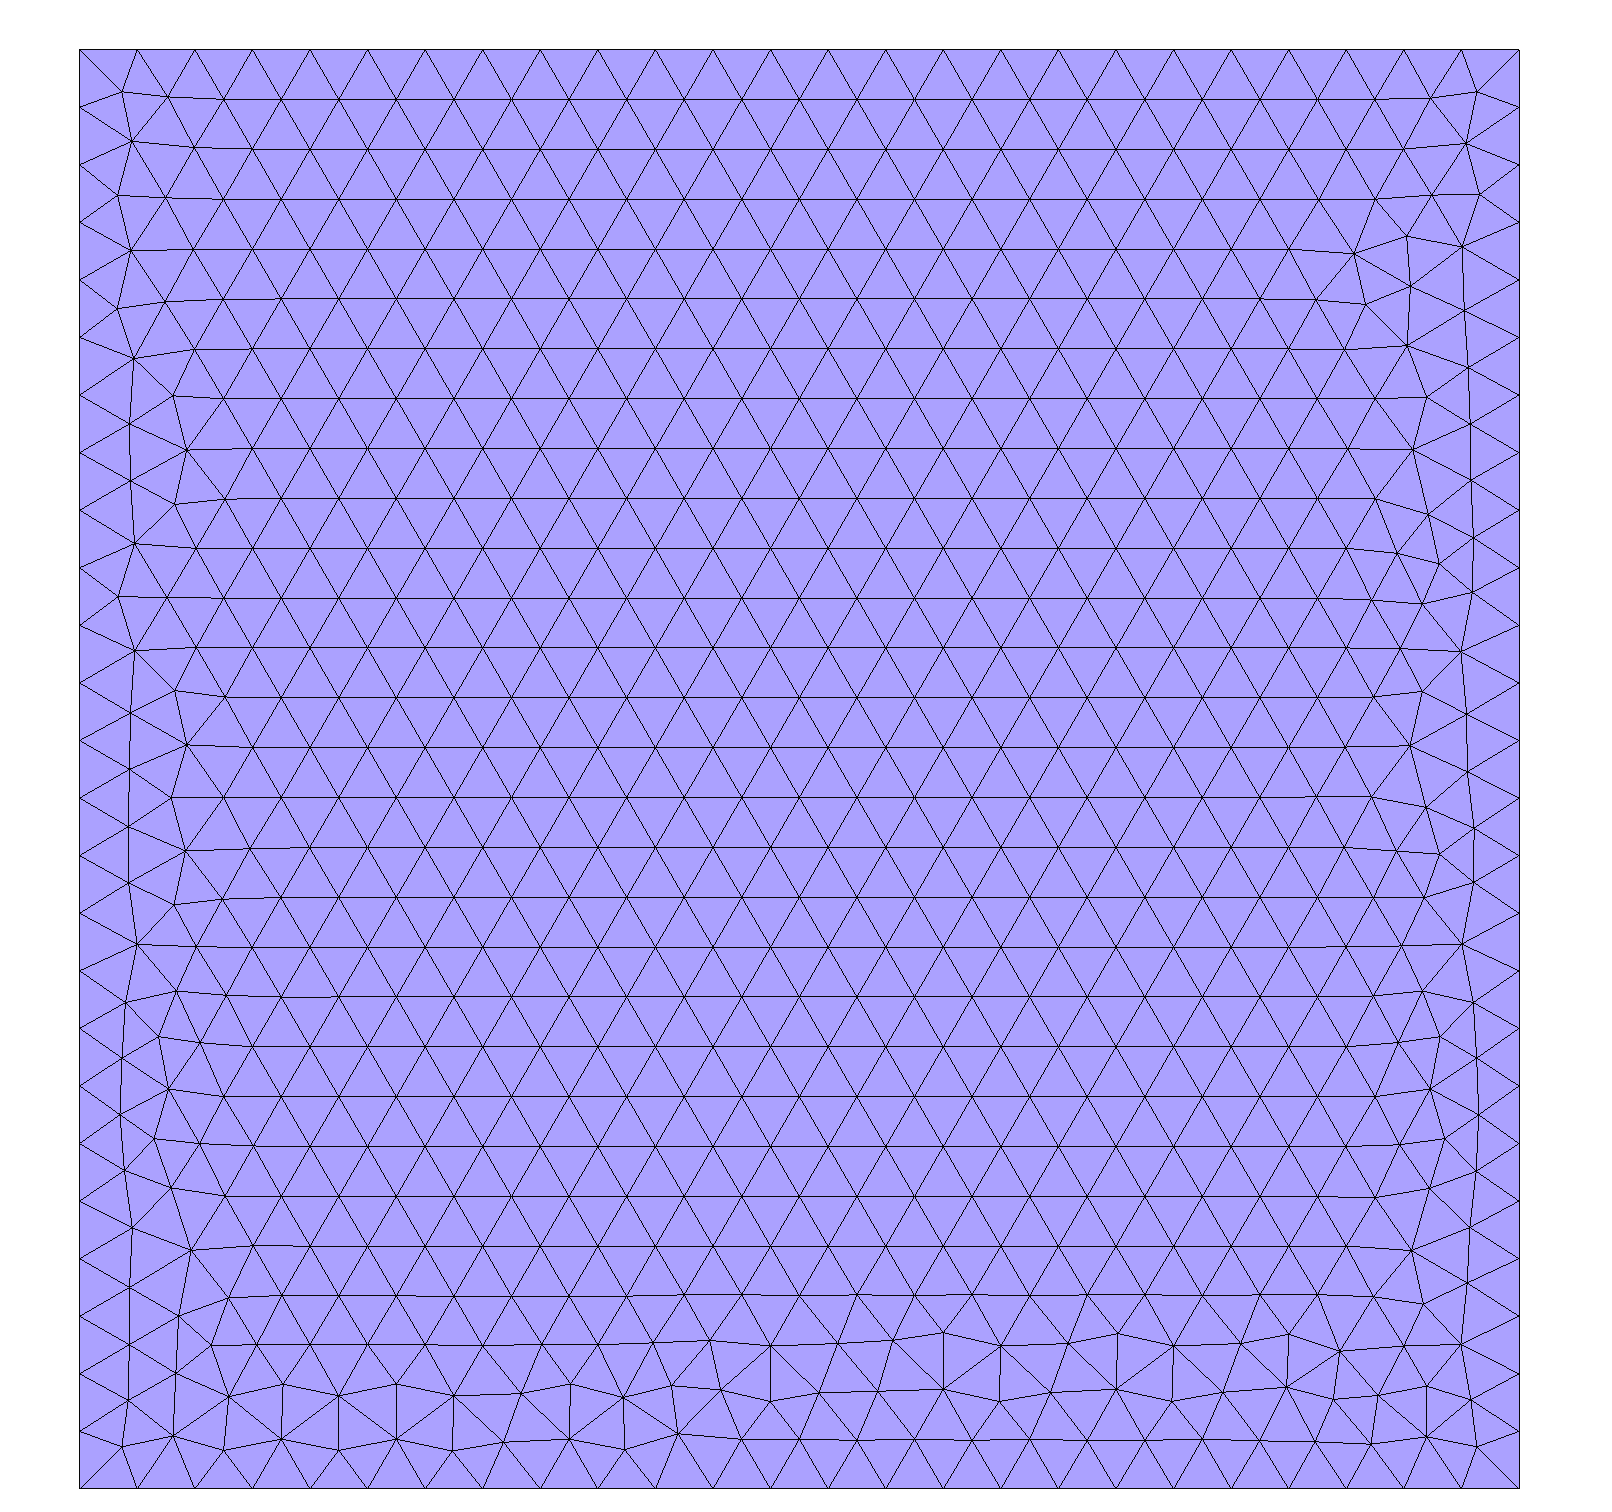
\includegraphics[width=0.4\textwidth]{images/square2d_M0.png}
  \caption{square2d\_M0.msh}
  \label{fig:mesh_square2d_M0}
  \end{figure}
  \columnbreak
  \begin{figure}[H]
  \centering
  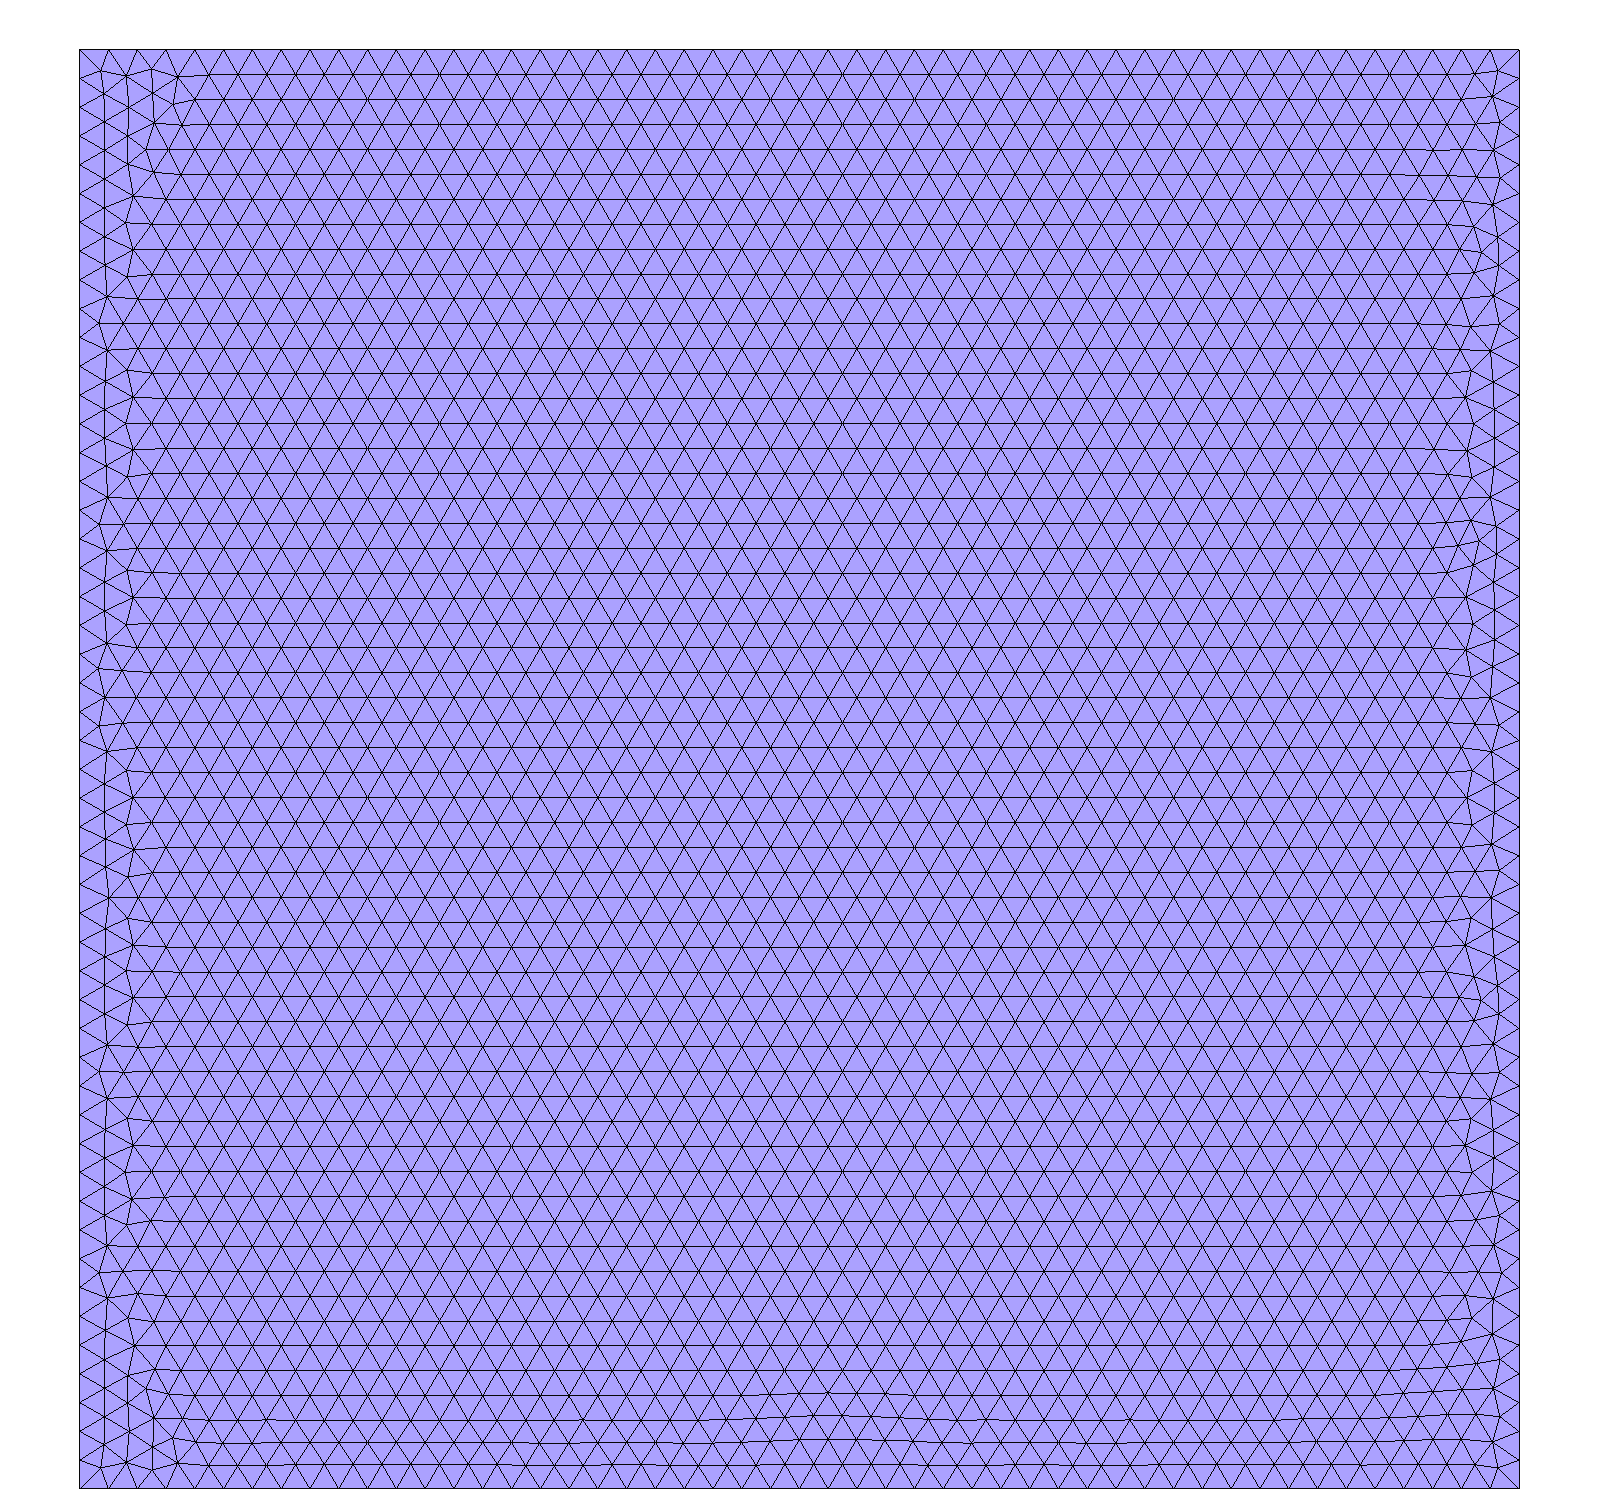
\includegraphics[width=0.4\textwidth]{images/square2d_M1.png}
  \caption{square2d\_M1.msh}
  \label{fig:mesh_square2d_M1}
  \end{figure}
  %\columnbreak
  \end{multicols}
\begin{multicols}{2}
  \begin{figure}[H]
  \centering
  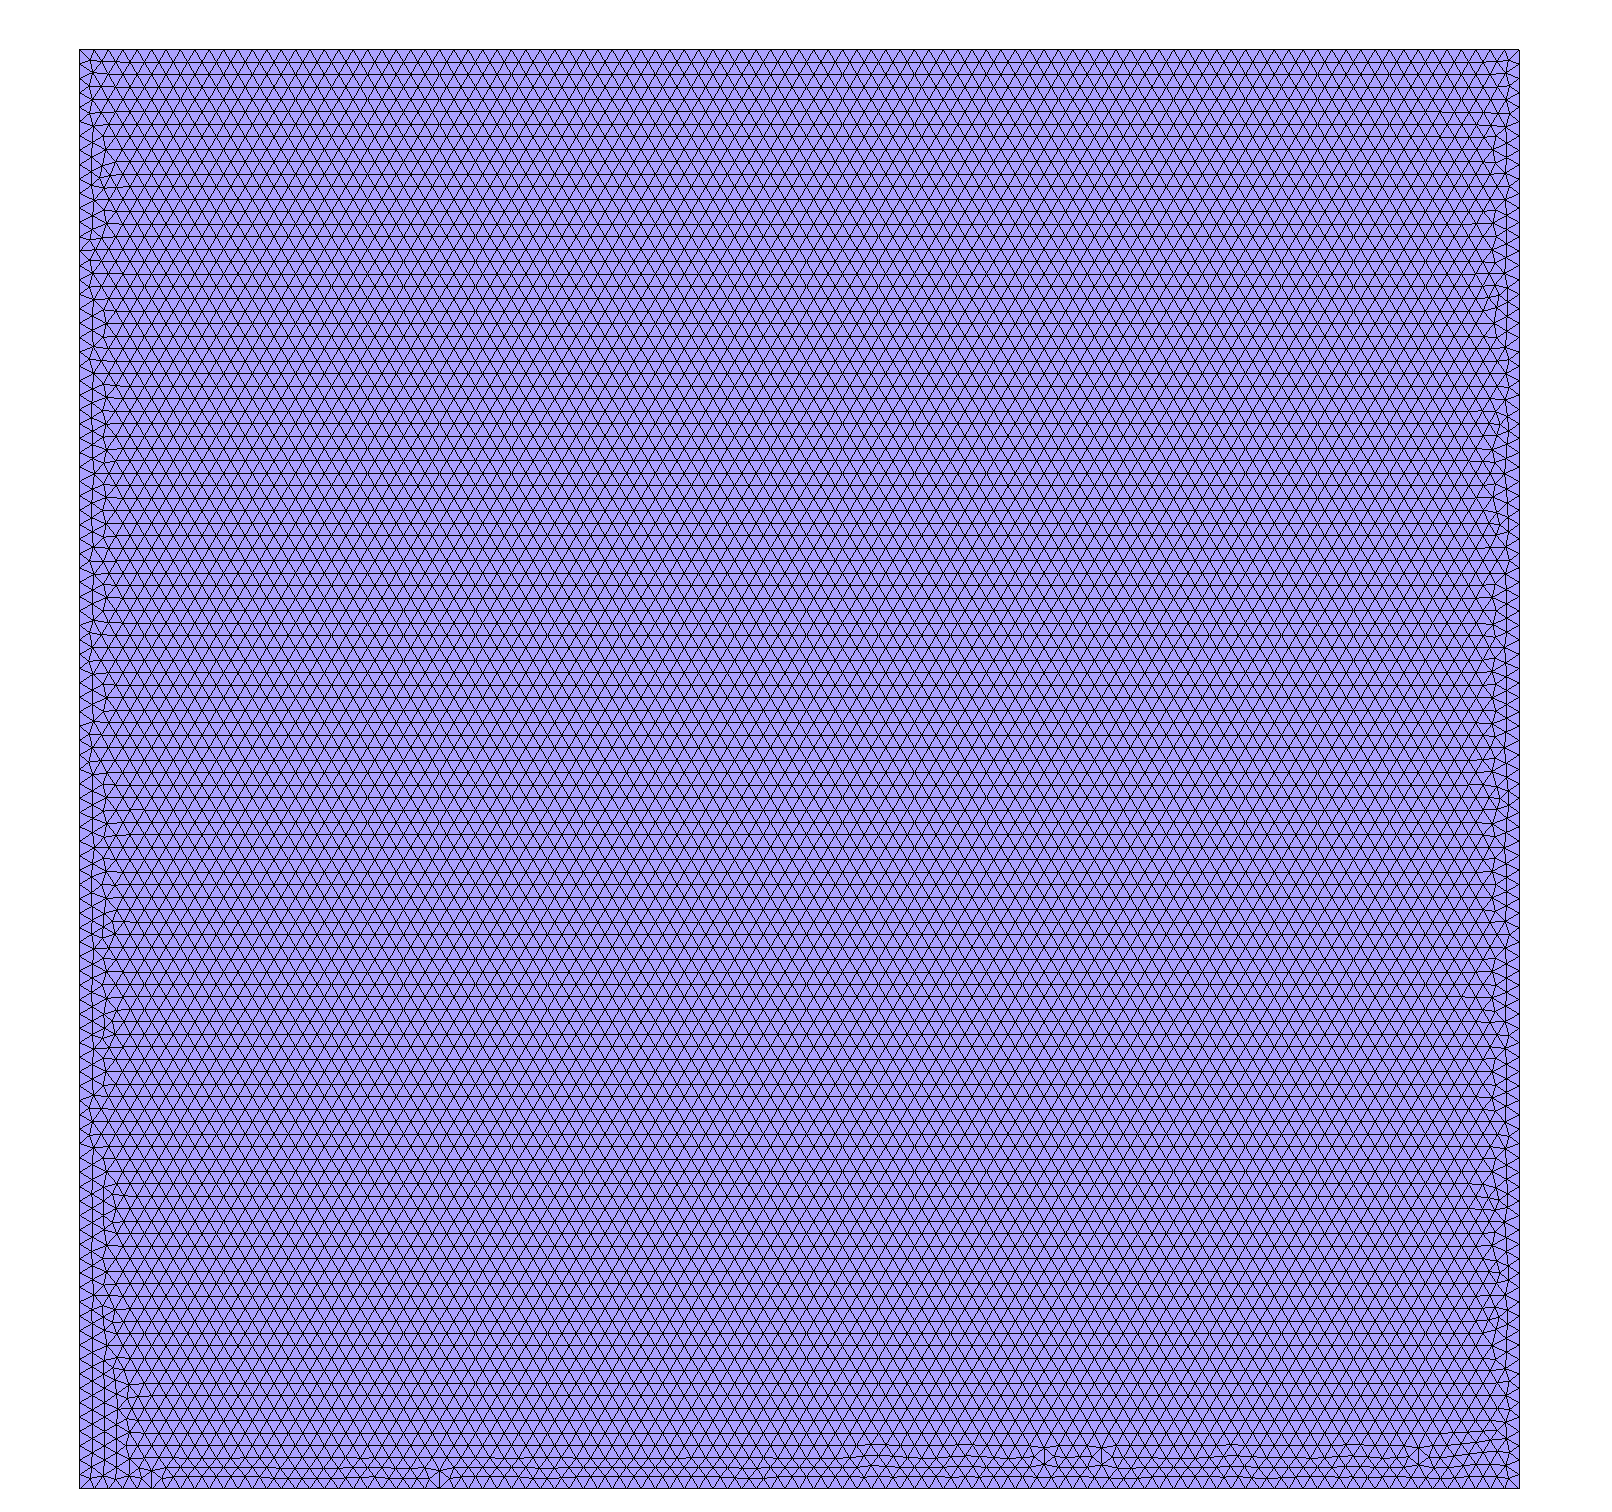
\includegraphics[width=0.4\textwidth]{images/square2d_M2.png}
  \caption{square2d\_M2.msh}
  \label{fig:mesh_square2d_M2}
  \end{figure}
  \columnbreak
  \begin{figure}[H]
  \centering
  
\includegraphics[width=0.4\textwidth]{images/square2d_perforated.png}
  \caption{square2d\_perforated.msh}
  \label{fig:mesh_square2d_perforated}
  \end{figure}
\end{multicols}


\paragraph{Notes:} We're going to use version 2 of the msh format, which is quite old but easier to load than the latest versions. The meshes supplied have been generated
square2d.geo and square\_perforated.geo files. The characteristic mesh size is defined by the h parameter at the beginning of the .geo file.
To generate a mesh from a .geo file, either open the software and export it in msh Version 2 ASCII format, or
command line: 
% write commande line
\begin{lstlisting}[language=bash]
$ gmsh -2 square2d.geo -format msh2 -o square2d.msh
\end{lstlisting}

\paragraph{}
To describe this file format, we'll consider the square2d\_4elt.msh file whose contents are shown below.
It represents the discretization of a square composed of just 4 triangles. In addition, the edges (i.e. segments) on the edge of the domain are also defined so that we can
the boundary conditions of the PDE. The 2 figures below illustrate the mesh and the numbering of points, edge segments and triangles.

\paragraph{}
\begin{minipage}[c]{0.4\linewidth}

\begin{mycpplistingInTabular}{square2d\_4elt.msh}
$\dollar$MeshFormat
2.2 0 8
$\dollar$EndMeshFormat
$\dollar$PhysicalNames
2
1 1 "Gamma"
2 2 "Omega"
$\dollar$EndPhysicalNames
$\dollar$Nodes
5
1 0 0 0
2 1 0 0
3 1 1 0
4 0 1 0
5 0.5 0.5 0
$\dollar$EndNodes
$\dollar$Elements
8
1 1 2 1 1 4 1
2 1 2 1 2 1 2
3 1 2 1 3 2 3
4 1 2 1 4 3 4
5 2 2 2 6 1 2 5
6 2 2 2 6 4 1 5
7 2 2 2 6 2 3 5
8 2 2 2 6 3 4 5
$\dollar$EndElements
\end{mycpplistingInTabular}

\end{minipage} \hfill
\begin{minipage}[c]{0.6\linewidth}
\begin{figure}[H]
  \centering
  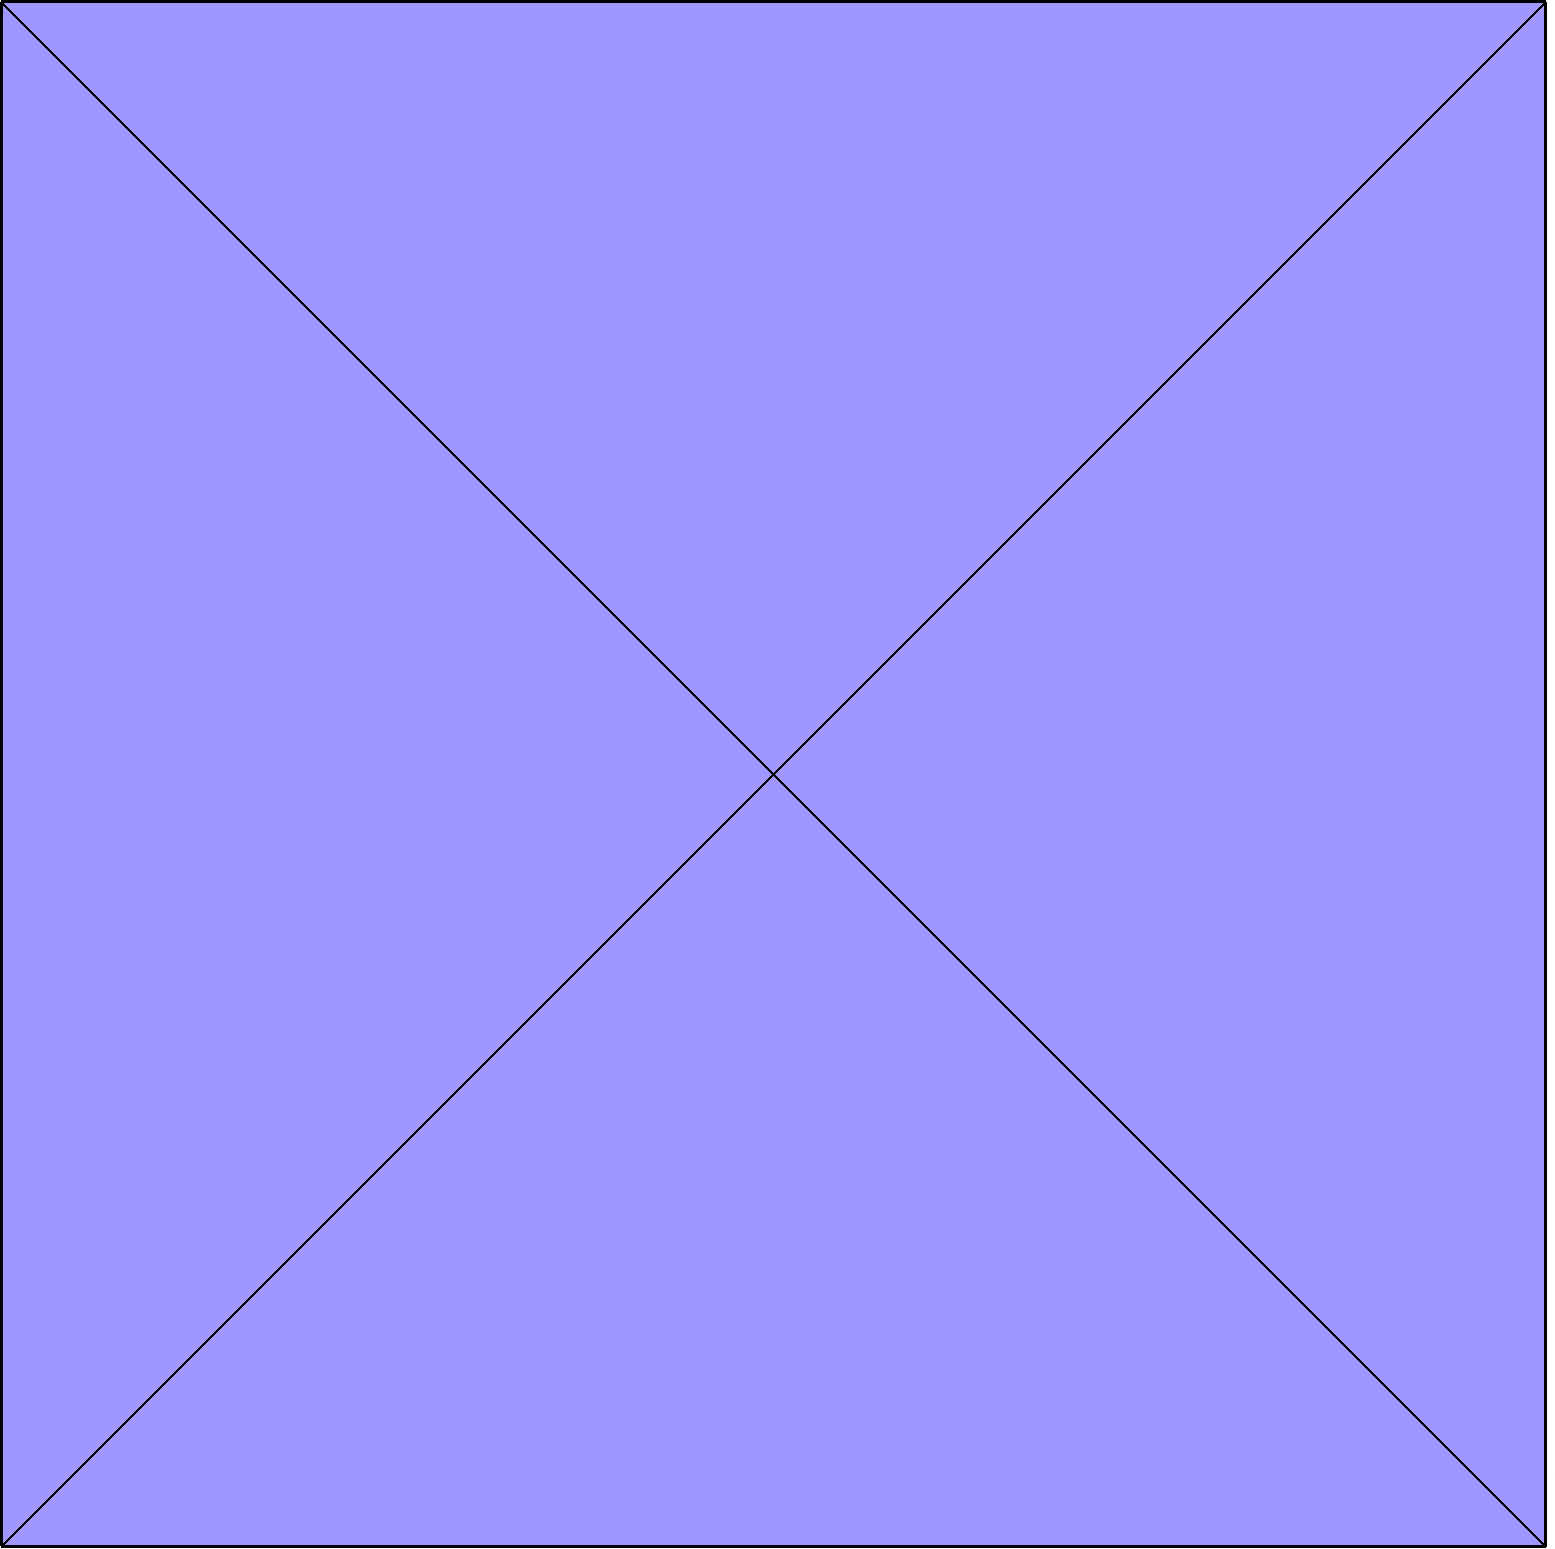
\includegraphics[width=0.4\textwidth]{images/square2d_4elt.png}
\end{figure}
\begin{figure}[H]
  \centering
  \vspace*{-0.05\textwidth}
  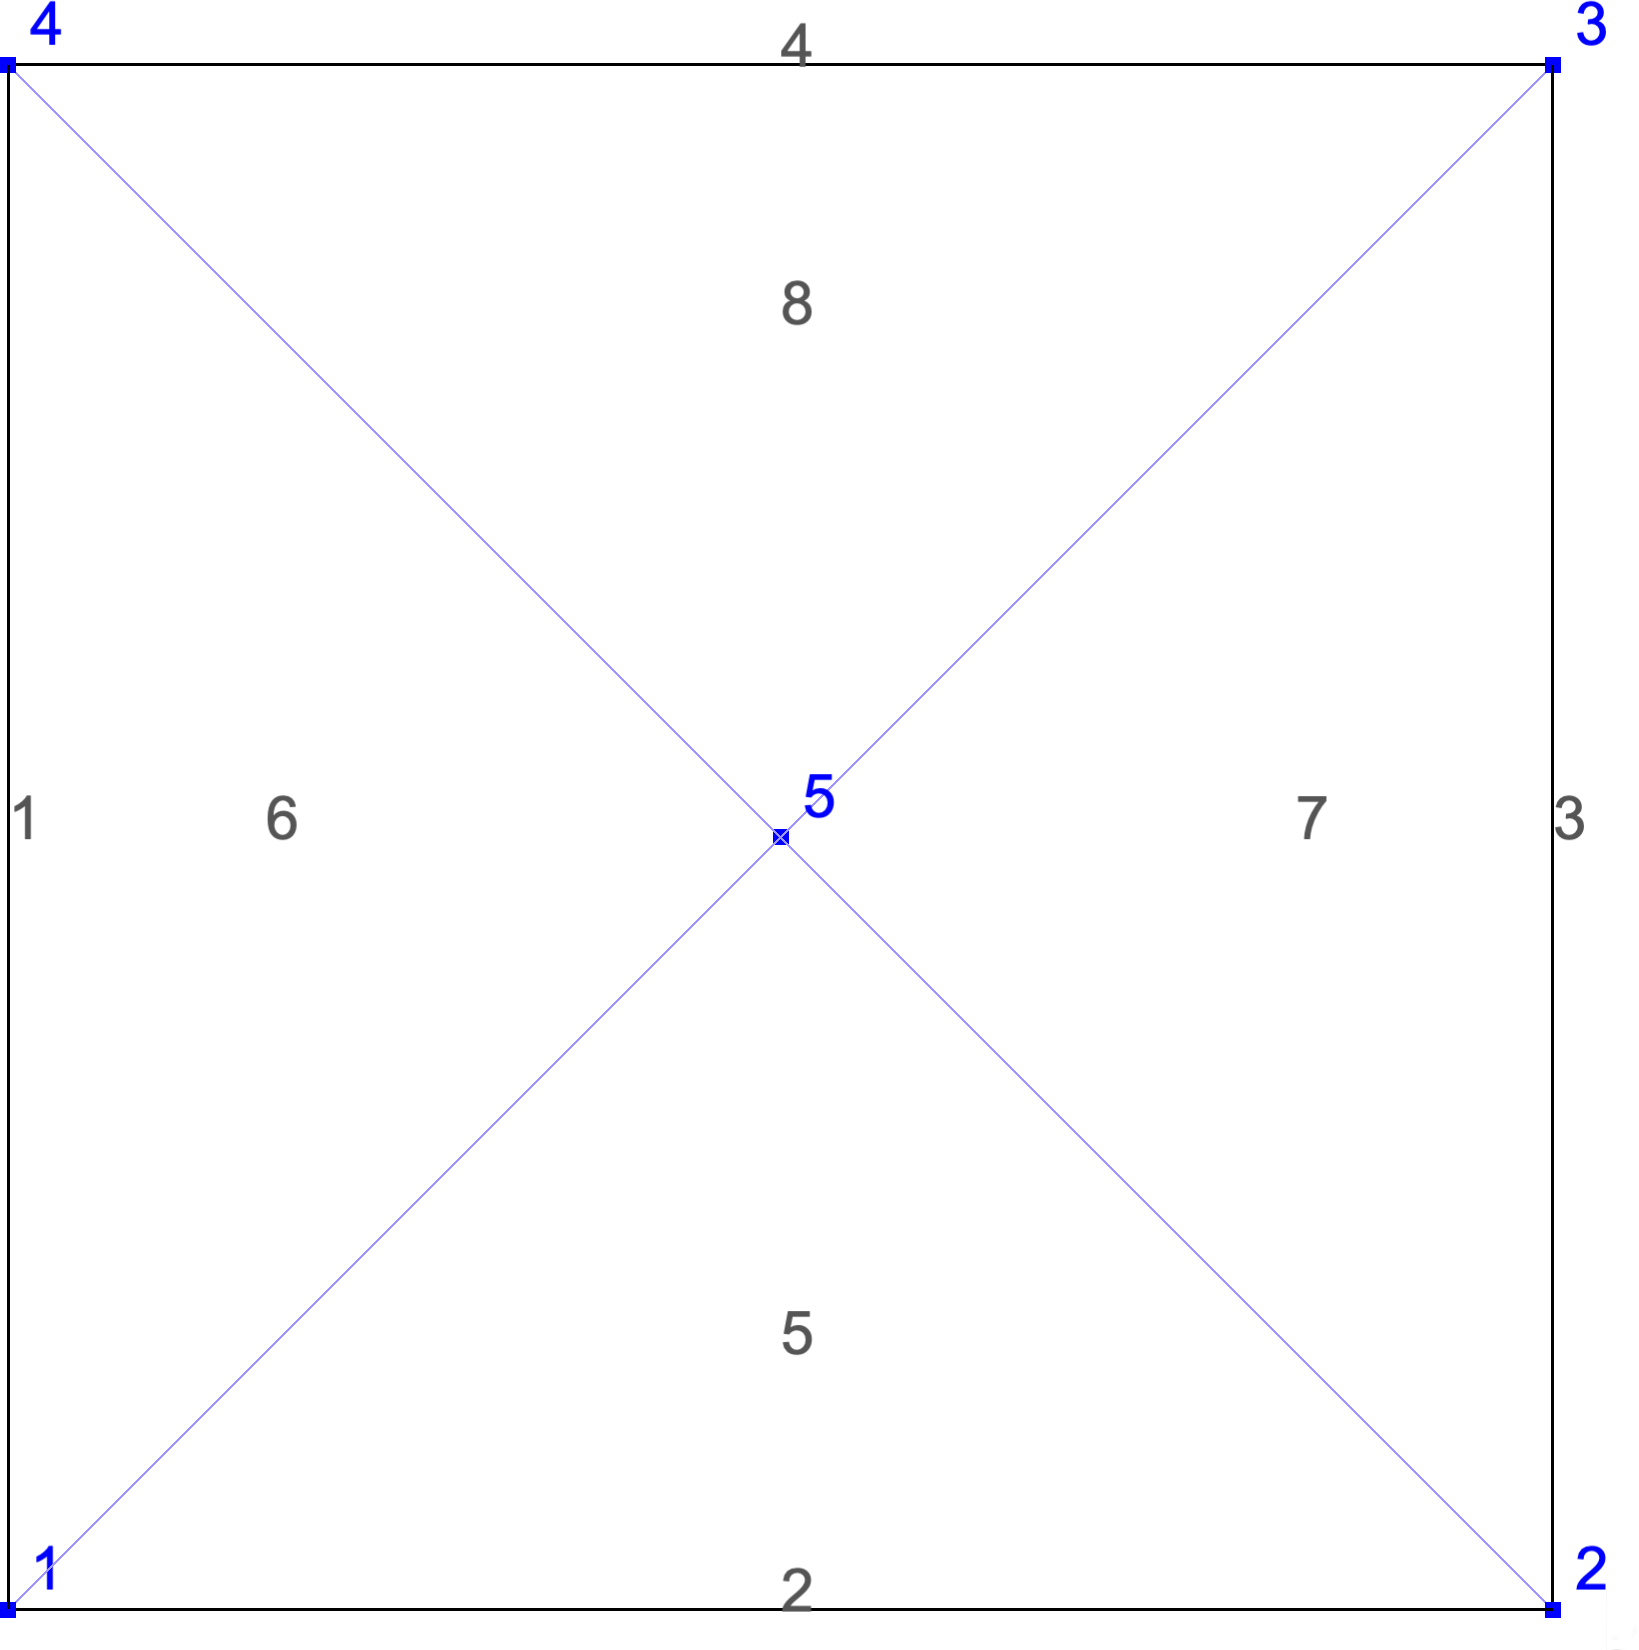
\includegraphics[width=0.4\textwidth]{images/square2d_4elt_numbering.png}
\end{figure}
\end{minipage}

\paragraph{}
We can see that this file is composed of 4 sections:
\begin{itemize}
\item \textbf{MeshFormat}: description of the msh format used. Here, check that the first argument 2.2. The other 2 values are not relevant to the project.
\item \textbf{PhysicalNames} : description of the physical markers of the mesh elements. A marker associates a character string with an integer, which is used in the element description.
  The first value is the number of markers. Then each line is made up of 3 values:
  \begin{enumerate}
  \item an integer for the element dimension (1 for segments, 2 for triangles)
  \item an integer representing the marker
  \item a character string associated with the marker
  \end{enumerate}
\item \textbf{Nodes}: description of the points present in the mesh. The first value represents the number of points.
  Then each line represents a point in the mesh with :
  \begin{itemize}
  \item the first number is a point identifier, in this case an integer.
  \item the other 3 values are the point's $x$, $y$ and $z$ coordinates. 
  \end{itemize}
\item \textbf{Elements} : a list of elements describing the mesh. For this project, we'll only be using two-dimensional meshes made up of segments and triangles.
  The first value is the number of elements to be described. Then each line represents the description of an element (segment or triangle) as follows:
  \begin{itemize}
  \item the first number is an element identifier, in this case an integer.
  \item the second value (an integer) is the element type. This value is 1 for segments and 2 for triangles.
  \item the third value (an integer) corresponds to the number of properties (or tags) associated with the element. Here, it's always 2.
  \item as the previous value will always be 2, we'll then have 2 integers. The first is the physical tag (see PhysicalNames section). The second is a geometry-related tag that we'll ignore.
  Finally, we'll have the identifiers of the points forming the element. Thus, there will be 2 numbers in the case of a segment and 3 numbers for triangles.
  \end{itemize}
\end{itemize}

\paragraph{Note:} Note that point or element identifiers start at 1 (not 0).

\paragraph{Objectives :}
Write a C++ program to load these meshes into memory. You'll then need to calculate the area of the mesh (by summing the area of each triangle) and the length of the edge of the domain.
The expected results are :
\begin{itemize}
\item for the square without perforation: area=1 and edge length=4
\item for the square with perforation: area $\approx$ 0.837725 and edge length $\approx$ 11.5086
\end{itemize}


\paragraph{Indications:}
Consider a triangle $T$ composed of the 3 vertices $A_1$, $A_2$ and $A_3$ which are represented respectively by the points $(x_1,y_1)$, $(x_2,y_2)$ and $(x_3,y_3)$.
The area of triangle $T$ is then given by the following relationship:

\begin{eqnarray*}
2 \mathrm{Area}(T) = \det \left(
  \begin{matrix}
    1 & x_1 & y_1 \\
    1 & x_2 & y_2 \\\\
    1 & x_3 & y_3
  \end{matrix}
  \right)
\end{eqnarray*}




\section{Post-Processing}

In this second section, we want to perform the following two post-processing operations:
\begin{enumerate}
\item Visualize a function/expression defined on a mesh using \textsc{ParaView} by knowing its values at the nodes (i.e. points) of the mesh.
  This function could be a solution to our PDE, which we'll deal with in Section 3.
\item Evaluate the integral of a function/expression on the mesh. Several methods known as quadrature formulas will be proposed, and the
  the choice of method will depend on the expression to be integrated.
\end{enumerate}

\subsection{View under \textsc{ParaView}}
ParaView software is widely used in scientific computing for its visualization and post-processing functions.
To do this, we're going to build a file in VTK format (compatible with \textsc{ParaView}) to export a mesh and one (or more) functions using these values at each point of the mesh.

\paragraph{}
To describe the VTK format, we'll use a mesh composed of 4 triangles. The exported function will be $f(x,y)=x^2+y^2$.
The VTK file to be generated for this mesh is supplied under the name square2d\_4elt.vtk. Try opening this file under \textsc{ParaView}.
We'll now describe the VTK format based on this file.
The first part of the file begins with a description of the format and type of data to be exported:
\begin{mycpplistingInTabular}{}
# vtk DataFile Version 2.0
my example
ASCII
DATASET UNSTRUCTURED_GRID
\end{mycpplistingInTabular}{}
The first line shows the version of the VTK file format.
The second line is a name given to the export (this name is not really important for our purposes).
The last 2 lines specify the data type.
This part will always be identical for all the exports we make in this project.

\paragraph{}
The next part lists all the points in the mesh:
\begin{mycpplistingInTabular}{}
POINTS 5 float
0 0 0
1 0 0
1 1 0
0 1 0
0.5 0.5 0
\end{mycpplistingInTabular}
The number 5 corresponds to the number of points and the keyword float represents the precision used by the software \textsc{ParaView}.
Next, we have 5 lines representing the $x$, $y$ and $z$ coordinates of each point. As we're using a 2d mesh, the $z$ coordinate will always be 0.
It's important to understand that each point is associated with a VTK point identifier (numbering in the VTK sense). The first point has an identifier equal to 0, the second to 1, etc...

\paragraph{}
The next 2 sections describe the elements (triangles) of the mesh. The first gives, for each element, the list of points
list of points describing the element (so here there will always be 3 point identifiers for a triangle):
\begin{mycpplistingInTabular}{}
CELLS 4 16
3 0 1 4
3 3 0 4
3 1 2 4
3 2 3 4
\end{mycpplistingInTabular}
After the CELLS keyword, we have the number of elements (i.e. the number of triangles in the mesh). The number 16 represents the number of values to be read in the rest of this section.
For each line, we have the description of a triangle, i.e. composed of 3 points, the first value appearing each time. Then we have the identifiers of the points making up the triangle
in VTK numbering (see commentary in previous section).
In this example, we have 4 triangles, each represented by 3 points, so the number 16 is equal to the number of triangles multiplied by 4.

The next section shows the type of element in relation to the previous description. As we're only dealing with triangles, the so-called VTK triangle type will always be equal to 5.
\begin{mycpplistingInTabular}{}
CELL_TYPES 4
5
5
5
5
\end{mycpplistingInTabular}
The number 4 represents the number of elements (triangles). Then simply add as many 5s as there are triangles in the mesh.


\paragraph{Hints:}
Now you can load this VTK file into \textsc{ParaView}, and you should be able to visualize the mesh.

\paragraph{}
Finally, we'll add the values of a function at each point of the mesh. Here we consider the function $f(x,y)=x^2+y^2$.
\begin{mycpplistingInTabular}{}
POINT_DATA 5
SCALARS toto float 1
LOOKUP_TABLE default
0
1
2
1
0.5
\end{mycpplistingInTabular}
In the first line, the number 5 represents the number of points.
The second line gives the function's characteristics. In this project, we'll be using only scalar functions (i.e., with a value in $\mathbb{R}$).
and whose float precision will be sufficient for visualization.
Consequently, the only parameter you'll be able to choose here is defined by the word toto, which will represent the function viewable under \textsc{ParaView} with this name.
You can then define several fields to be visualized in this format by adding similar sections but changing this name.
The third line must be added, but don't worry about its role.
The following lines represent the value of the function at each point of the mesh (respecting VTK numbering).

\paragraph{Objectives:} Enable your C++ program to generate VTK files from a mesh and the definition of an expression for the $f$ function. This expression
will be evaluated at each point of the mesh. A VTK file export tool will need to be developed, with a mesh parameter, a function evaluated at the mesh nodes
and a function name that will appear under \textsc{ParaView}. The saved file can be named with this name followed by the suffix .vtk (e.g. toto.vtk).
Figures \ref{fig:mesh_square2d_M2_export} and \ref{fig:mesh_square2d_perforated_export} illustrate a visualization with \textsc{ParaView} on the mesh square2d\_M2.msh and square2d\_perforated.msh.

%\newpage
\begin{multicols}{2}
  \begin{figure}[H]
    \centering
    
\includegraphics[width=0.4\textwidth]{images/square2d_M2_export.png}
    \caption{$f(x,y)=x^2+y^2$}
    \label{fig:mesh_square2d_M2_export}
  \end{figure}
  \columnbreak
  \begin{figure}[H]
    \centering
    
\includegraphics[width=0.4\textwidth]{images/square2d_perforated_export.png}
    \caption{$f(x,y)=(x-0.5)^2+(y-0.5)^2$}
    \label{fig:mesh_square2d_perforated_export}
  \end{figure}
\end{multicols}


\subsection{Numerical integration}

Numerical integration is a technique for performing exact or approximate integral calculations, depending on the type of expression to be integrated.
Most numerical integration formulas are derived from polynomial interpolation methods. Calculating the integral of a function
is approximated by the exact calculation of the integral of a polynomial interpolating this function at certain points $\left\{x_q\right\}_{q=1}^p$, called integration points.
This gives a general form for numerical quadratures on a $K$ triangle:
\begin{equation*}
  \int_K f(x,y) dxdy \approx \sum_{q=1}^p w_q f(x_q)
\end{equation*}
with coefficients $w_q$ called weights of the quadrature formula.

\paragraph{}
The cost of a quadrature formula is measured by the number of evaluations of the function $f$ required, i.e. by the number of integration points.
The precision of a numerical integration formula is defined by the maximum polynomial order for which the integration of a polynomial is exact.
A quadrature formula is said to be of order $k$ if the maximum polynomial order is $k$. 

\paragraph{}
Integrating an expression over our discretized computational domain $\Omega_h$ boils down to integrating the expression over each mesh element.
We thus have :
\begin{equation*}
  \int_{\Omega_h} f = \sum_{e=1}^{N_e} \int_{K_e} f
\end{equation*}

In the case of triangles, the integration points are expressed using the barycentric coordinates $\lambda_1$, $\lambda_2$ and $\lambda_3$.
If we consider a triangle defined by 3 vertices $A_1$, $A_2$ and $A_3$ which are represented respectively by the points $(x_1,y_1)$, $(x_2,y_2)$ and $(x_3,y_3)$, then
a point $(x,y)$ can be expressed in terms of its barycentric coordinates as follows:

\begin{eqnarray*}
  x &=& \lambda_1 x_1 + \lambda_2 x_2 + \lambda_3 x_3 \\
  y &=& \lambda_1 y_1 + \lambda_2 y_2 + \lambda_3 y_3
\end{eqnarray*}


Remember that barycentric coordinates must verify :
\begin{equation*}
  \lambda_1 + \lambda_2 + \lambda_3 = 1
\end{equation*}


We'll now present a few quadrature formulas, each time defining the barycentric coordinates and associated weights.
S is the area of the triangle over which the integration is performed.

\paragraph{Quadrature of order 1 :} 1 integration point
\begin{itemize}
\item barycentric coordinates: $\left(\frac{1}{3},\frac{1}{3},\frac{1}{3}\right)$.
\item weight: $S$
\end{itemize}

\paragraph{Quadrature of order 2:} 3 integration points
\begin{itemize}
\item coord. barycentriques : $\left(\frac{2}{3},\frac{1}{6},\frac{1}{6}\right)$, $\left(\frac{1}{6},\frac{2}{3},\frac{1}{6}\right)$, $\left(\frac{1}{6},\frac{1}{6},\frac{2}{3}\right)$
\item poids : the 3 weights are equal to $\frac{1}{3} S$
\end{itemize}

\paragraph{Quadrature of order 3:} 4 integration points
\begin{itemize}
\item coordin. barycentric: $\left(\frac{1}{3},\frac{1}{3},\frac{1}{3}\right)$,
  $\left(\frac{3}{5},\frac{1}{5},\frac{1}{5}\right)$,
  $\left(\frac{1}{5},\frac{3}{5},\frac{1}{5}\right)$ ,
  $\left(\frac{1}{5},\frac{1}{5},\frac{3}{5}\right)$
\item weights: the first with $-\frac{9}{16} S$ and the other 3 with $\frac{25}{48} S$
\end{itemize}

\paragraph{Objectives:} Implement a function/class for calculating an integral with a parameter allowing you to choose one of the quadrature formulas presented above.
You'll need to test the formulas for correctness, using polynomial integration as an expression on the domain without perforation. The result will then be known.
Also analyze the behavior of quadratures on non-polynomial expressions as a function of refinement (i.e. by comparing on meshes M0, M1 and M2).



\section{A finite element solution method}

In this third section, we'll use a finite element method to solve the problem presented in the introduction, and find an approximate solution to the PDE.
The description of the method will be brief, and a number of mathematical details will not be explained.
However, you will have the essentials to implement this method in your program.

In the following, we assume that we have a mesh of the $\Omega$ domain formed by $N_e$ triangles, which we denote $\Omega_h$.
These triangles are defined using $N_p$ points (all different), denoted by the set of coordinates $\left\{ (x_i,y_i) \right\}_{i=1}^{N_p}$.

\subsection{Approximation by finite Lagrange element $\mathbb{P}_1$}

To begin with, we need to define an approximation space for the solution of the PDE, which we'll call $V_h$.
This will be the space of functions that are continuous on the mesh and affine on each triangle of the mesh. This is expressed by :

\begin{equation*}
  V_h = \left\{ v \in C^0(\Omega) \text{ such that } v_{|K_e} \in \mathbb{P}_1, \ \forall e=1...N_e \right\}
\end{equation*}

\paragraph{}
%\begin{minipage}[l]{0.7\linewidth}
\begin{wrapfigure}{R}{0.4\textwidth}
%begin{figure}[H]
  \centering
  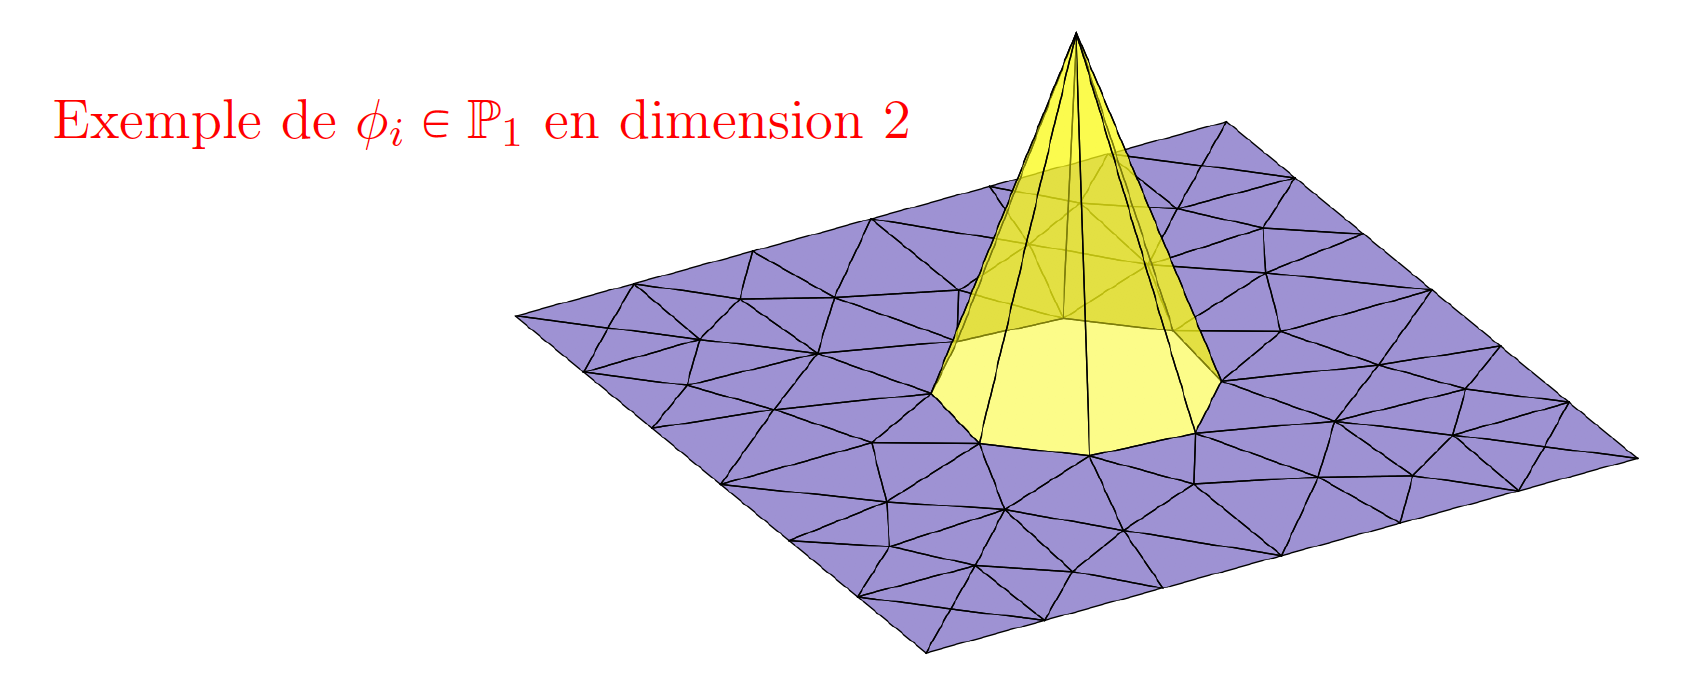
\includegraphics[width=0.38\textwidth]{images/fonction_base_P1.png}
%\end{figure}
\end{wrapfigure}
The dimension of $V_h$ is equal to the number of mesh points $N_p$. A basis of this space is constructed by choosing the $N_p$ functions $\phi_i$ of $V_h$.
which verify
\begin{equation*}
  \phi_i(x_j,y_j) = \delta_{ij}, \quad \forall i=1...N_p \text{ and } \forall j=1...N_p
\end{equation*}
The figure opposite shows an example of one of $V_h$'s basic functions. All these functions are of the same form, a function $\phi_i$ is worth 1 on node $x_i,y_i$ and zero on all other nodes.
%\end{minipage} \hfill
%\begin{minipage}[c]{0. 3\linewidth}
%\end{minipage}
%\paragraph{}
Thus, a function $u_h \in V_h$ will be determined by its values at the mesh nodes by the following relationship:
\begin{equation*}
  u_h(x,y) = \sum_{i=0}^{N_p} u_i \Phi_i (x,y)
\end{equation*}
with $\left\{u_i \equiv u(x_i,y_i)\right\}_{i=1}^{N_p}$ the set of values to be determined. These values are called degrees of freedom.


\paragraph{}
Let K be a triangle composed of the 3 vertices $A_1$, $A_2$ and $A_3$ which are represented respectively by the points $(x_1,y_1)$, $(x_2,y_2)$ and $(x_3,y_3)$.
The restrictions of the basis functions in the K-element are referred to as shape functions.
In each triangle, there are only 3 non-zero basis functions. The restrictions of these 3 basis functions in triangle K are denoted by $\phi_1^K$, $\phi_2^K$, $\phi_3^K$. These are
three polynomial functions of degree 1, taking the value 1 at one vertex and zero at the other 2.
The index 1, 2 or 3 of the shape functions represents the vertex for which the value is 1.
For example, $\phi_1^K$ is the affine function that has a value of 1 at vertex $A_1$ and zero at vertices $A_2$ and $A_3$.
Thus, the shape functions in a triangle K are defined by the following expressions:
\begin{eqnarray*}
 \phi_1^K(x,y) = \frac{x_2 y_3 - x_3 y_2 + x (y_2-y_3)+y(x_3-x_2)}{2 Area(T)} \\
 \phi_2^K(x,y) = \frac{x_3 y_1 - x_1 y_3 + x (y_3-y_1)+y(x_1-x_3)}{2 Area(T)} \\
 \phi_3^K(x,y) = \frac{x_1 y_2 - x_2 y_1 + x (y_1-y_2)+y(x_2-x_1)}{2 Area(T)} \\
\end{eqnarray*}


%% $u_h(x,y) = u_1 \phi_1(x,y) + u_2 \phi_2(x,y) + u_3 \phi_3(x,y)$
%% $u_h(x,y) = \sum_{i=0}^{N_p} v(x_i,y_i) \Phi_i (x,y) $

\subsection{Discrete variational formulation}

To solve the PDE presented in the introduction using the finite element method, we also need to transform this problem into a so-called variational formulation.
To do this, we need to introduce the following approximation spaces:
\begin{equation*}
  V_{0h} = \left\{ v \in V_h \ | \ v=0 \text{ on } \Gamma \right\} \text{ and } V_{gh} = \left\{ v \in V_h \ | \ v=g \text{ on } \Gamma \right\}
\end{equation*}

After manipulating the PDE, the discrete variational formulation is then given by the following problem:
\begin{eqnarray}
\left\{
  \begin{aligned}
     &\text{Find $u_h \in V_{gh}$ such that } \\
    &\int_{\Omega_h} \nabla u_h \cdot \nabla v = \int_{\Omega} f \ v, \quad \forall v \in V_{0h}
  \end{aligned}
  \right.
\end{eqnarray}


We denote by $I_i$ the set of indices of nodes in the mesh corresponding to an unknown value, i.e. not touching the edge.
$I_b$ denotes the set of indices of nodes in the mesh that lie on $\Gamma$, i.e. touching the edge.
By writing $u_h$ with the basis functions of $V_h$ space, this formulation can be expressed as the combination of the following 2 statements:
\begin{eqnarray*}
&\bullet& \left\{
  \begin{aligned}
    &\text{Find the values $u_j$ for $j \in I_i$ such that } \\
    & \sum_{j= 1}^{N_p} \left( \int_{\Omega_h} \nabla \phi_j \cdot \nabla \phi_i \right) u_j= \int_{\Omega_h} f \ \phi_i, \quad \forall i \in I_i
  \end{aligned}
  \right. \\
%% \end{eqnarray*}
%% \begin{eqnarray*}
&\bullet& \left\{
  \begin{aligned}
    &\text{Impose $u_j$ values for $j \in I_b$ such that } \\
    & u_j = g(x_j,y_j)
  \end{aligned}
  \right.
\end{eqnarray*}


We obtain a system of $N_p$ equations with $N_p$ unknowns, where $N_p$ designates the number of mesh points.
This system is written in matrix form
\begin{equation*}
  A U = F
\end{equation*}
where the entries for the matrix A and the second-member vector F are given by :
\begin{align*}
  A_{ij} &= \int_{\Omega_h}  \nabla \phi_j \cdot \nabla \phi_i = \sum_{e=1}^{N_e} \int_{K_e} \nabla \phi_j \cdot \nabla \phi_i ,\quad \forall i \in I_i, \forall j=1...N_p \\
  A_{ii} & = 1, \quad \forall i \in I_b \\\\
  F_i &= \int_{\Omega_h} f \ \phi_i = \sum_{e=1}^{N_e} \int_{K_e} f \ \phi_i , \quad \forall i \in I_i \\\\
  F_i &= g(x_i,y_i), \quad \forall i \in I_b \\\\
\end{align*}

\subsection{Assembly algorithm}

As you can see, the A matrix is very sparse, as many of its coefficients are zero.
This is due to the choice of $\phi_i$ basis functions, which have limited support.
Assembling the matrix A and vector F using the finite element method boils down to assembling so-called elementary matrices and vectors, as they are calculated for each of the mesh elements. 
Thus, for each triangle K of the mesh, the elementary matrix $A_k$ and elementary vector $F_k$ are evaluated as follows:
\begin{equation*}
A_K = \left(
  \begin{matrix}
    \displaystyle \int_K \nabla \phi_1^K \cdot \nabla \phi_1^K & \displaystyle \int_K \nabla \phi_1^K \cdot \nabla \phi_2^K & \displaystyle \int_K \nabla \phi_1^K \cdot \nabla \phi_3^K \\
    \displaystyle \int_K \nabla \phi_2^K \cdot \nabla \phi_1^K & \displaystyle \int_K \nabla \phi_2^K \cdot \nabla \phi_2^K & \displaystyle \int_K \nabla \phi_2^K \cdot \nabla \phi_3^K \\
    \displaystyle \int_K \nabla \phi_3^K \cdot \nabla \phi_1^K & \displaystyle \int_K \nabla \phi_3^K \cdot \nabla \phi_2^K & \displaystyle \int_K \nabla \phi_3^K \cdot \nabla \phi_3^K
  \end{matrix}
  \right)
  \text{ and }
  F_K = \left(
  \begin{matrix}
    \displaystyle \int_K f \phi_1^K \\
    \displaystyle \int_K f \phi_2^K \\
    \displaystyle \int_K f \phi_3^K
  \end{matrix}
  \right)
\end{equation*}




\begin{algorithmic}[1]
  \Require $A$ a matrix and $F$ a vector, each set to zero.
  \For{$e=1 \textbf{ to } N_e$}
  \State Calculate elementary matrix $A_{K_e}$.
  \State Elementary vector calculation $F_{K_e}$.
  \For{$s=1 \textbf{ to } 3$}
  \State $i = \Call{GlobalDof}{K_e,s}$
  \For{$t=1 \textbf{ to } 3$}
  \State $j = \Call{GlobalDof}{K_e,t}$
  \State $A(i,j) = A(i,j) + A_{K_e}(s,t)$
  \EndFor
  \State $F(i) = F(i) + F_{K_e}(s)$
  \EndFor
  \EndFor
  \For{$i \in I_b$}
  \For{$j=1 \textbf{ to } N_p$}
  \State $A(i,j)=0$
  \EndFor
  \State $A(i,i)=1$
  \State $F(i)=g(x_i,y_i)$
  \EndFor
\end{algorithmic}

In this algorithm, you'll find a function called \textsc{GlobalDof}. It takes 2 parameters as arguments: a triangle in the mesh and the index of a vertex in this triangle.
The function will then return the identifier of the global degree of freedom as an integer.
In our case, this will correspond to the identifier of the point in the mesh, and will therefore be between 1 and $N_p$ inclusive.
However, you need to be careful with C++ data structures (such as arrays, vectors and matrices \textsc{Eigen}). These have indices starting at zero, not 1.

In addition, the second part of the algorithm (lines 13 to 19) takes into account Dirichlet-type boundary conditions. Noting $I_b$, the set of degrees of freedom at the edge,
this method consists in modifying the $I_b$ rows of the $A$ matrix, as well as the values of the $F$ vector at the $I_b$ indices. To do this, all the entries in these rows must be set to zero, except for
The $F$ vector is modified by setting the value defined by the boundary condition. This technique is known as the elimination method.


\subsection{Problem solution}

To solve the system $A U = F$, we need to invert the potentially large but sparse matrix $A$.
Many techniques exist, either by explicitly calculating the inverse, or by using an iterative method.
However, we won't be implementing such a procedure, but rather using the \textsc{Eigen} library. \href{http://eigen.tuxfamily.org/dox/}{\color{shellpromptcolor} http://eigen.tuxfamily.org/dox/}.
It provides functionality for describing dense matrices, sparse matrices and vectors.
You'll need to use :
\begin{itemize}
\item Dense matrices for elementary matrices $A_k$.
\item Sparse matrices for the global matrix $A$.
\item The vectors for the elementary vectors $F_k$ and the global vector $F$.
\end{itemize}

This library also includes several solvers for solving the linear system.
Once solved by \textsc{Eigen}, you'll obtain the vector $U$ representing the finite element approximation of the problem.
Each $u_i$ value corresponds to the value of the solution at point $(x_i,y_i)$.

\subsection{Applications}

\subsubsection{Constant source term}

Initially, we will be interested in solving the PDE using a constant source term $f$, equal to 1.
In addition, we'll impose homogeneous Dirichlet conditions, i.e. $u=0$ on the edge.
This translates into the search for a function $u$ satisfying the following system:

\begin{eqnarray*}
\left\{
  \begin{aligned}
    - \Delta u &= 1 \quad \text{ in } \Omega \\
    u &= 0 \quad \text{ on } \Gamma
  \end{aligned}
  \right.
\end{eqnarray*}

Figures \ref{fig:res_square2d_M2} and \ref{fig:res_square2d_perforated} illustrate the numerical solutions obtained using this finite element method.
These visualizations were produced with \textsc{ParaView} using the \textit{Rainbow Desaturated} color scheme.

\begin{multicols}{2}
  \begin{figure}[H]
  \centering
  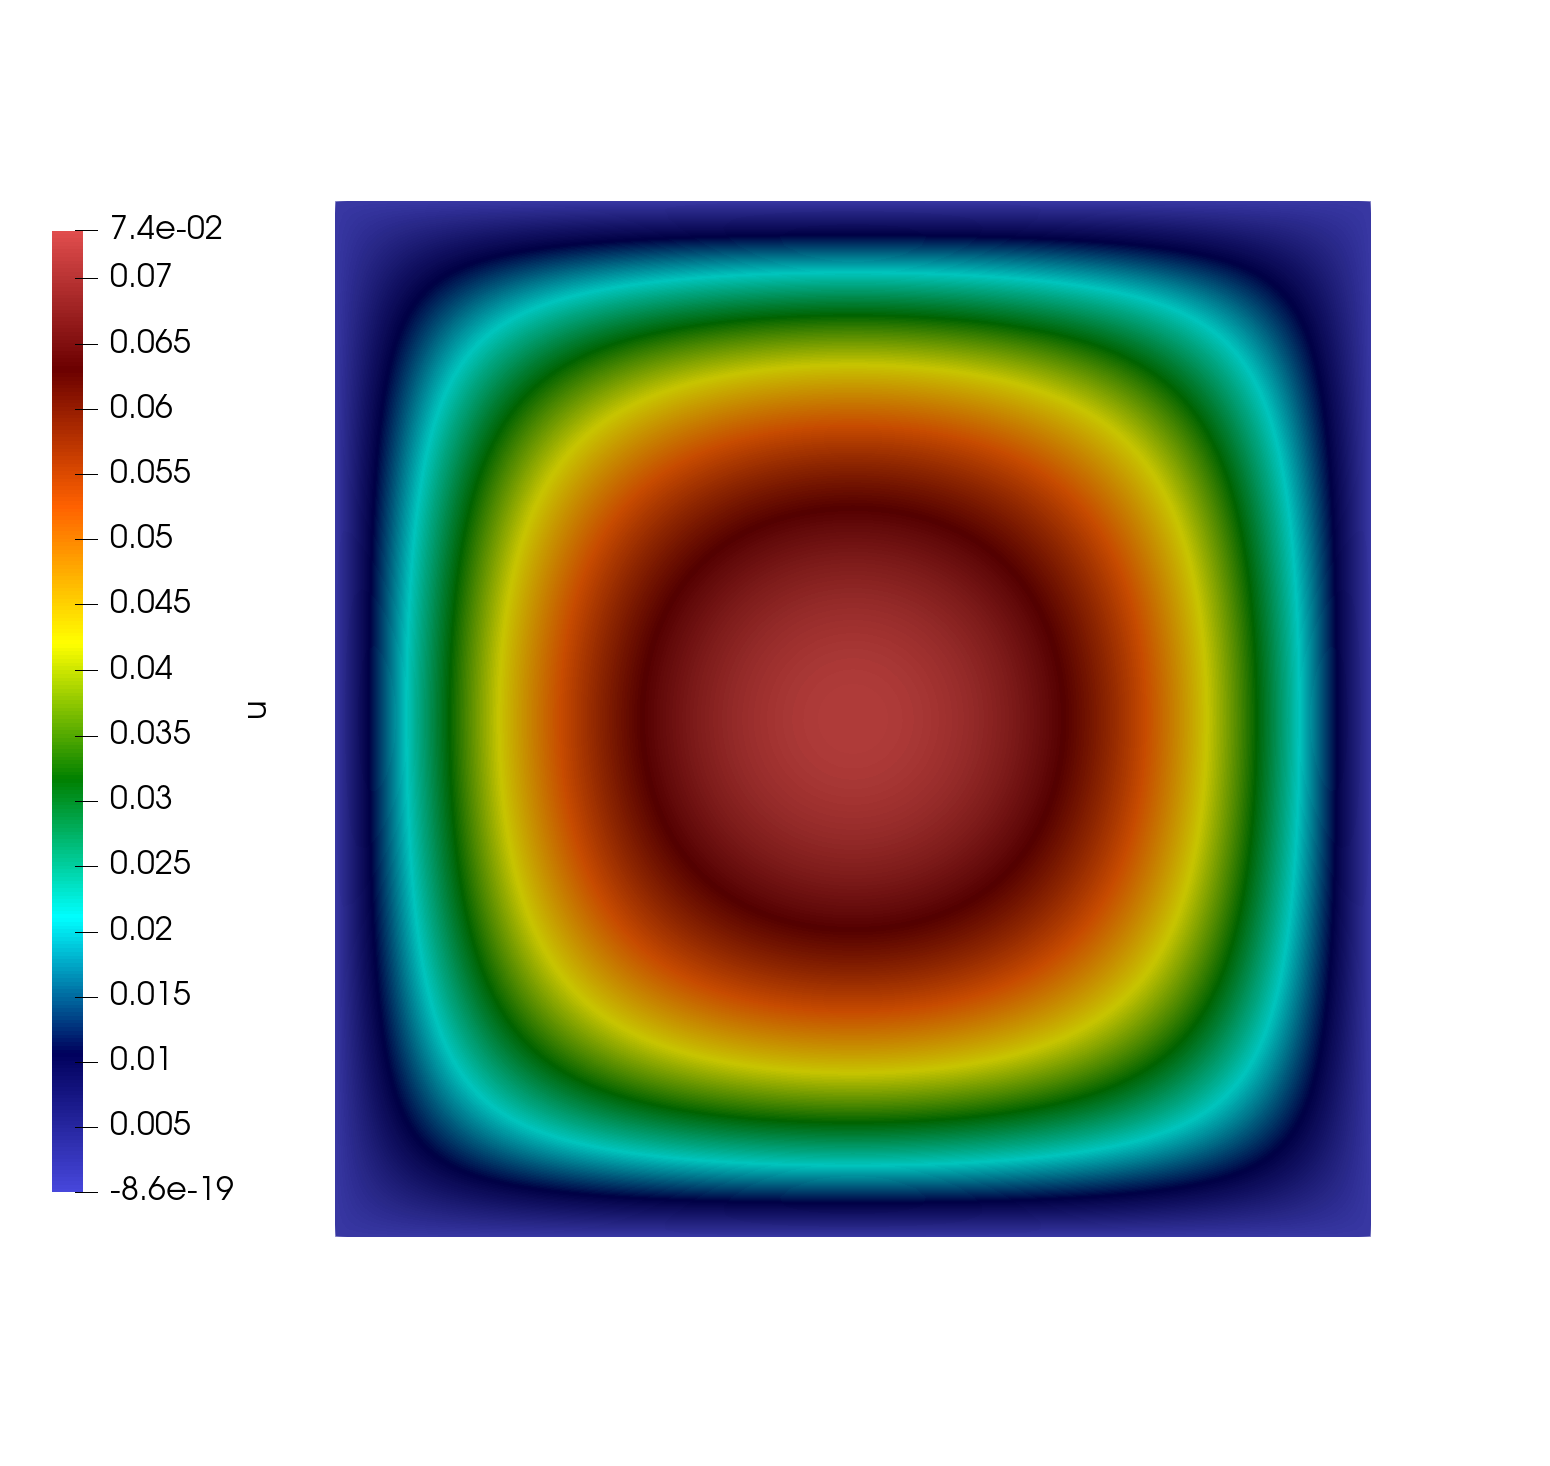
\includegraphics[width=0.4\textwidth]{images/resultat_f1_nonperfo.png}
  \caption{square2d\_M2. msh}
  \label{fig:res_square2d_M2}
  \end{figure}
  \columnbreak
  \begin{figure}[H]
  \centering
  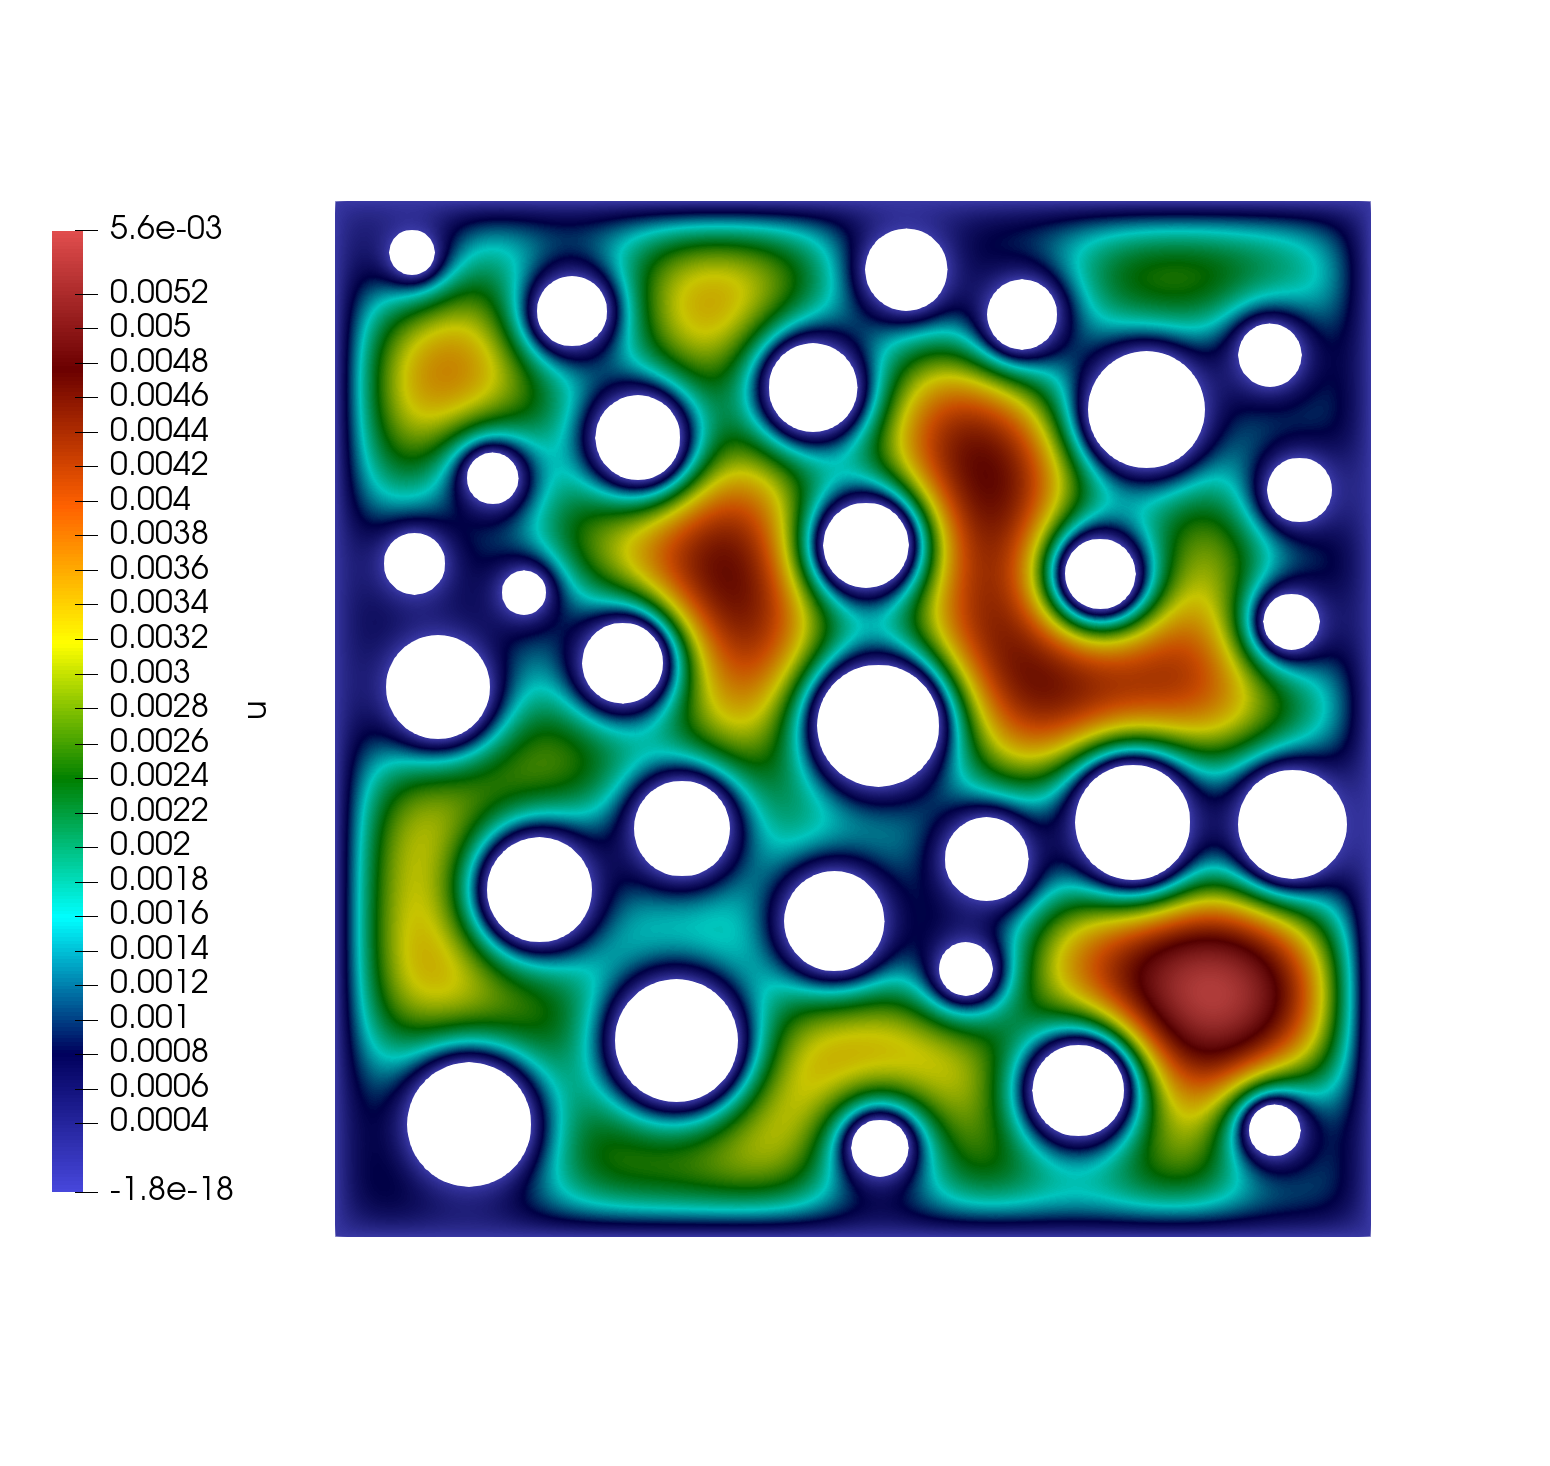
\includegraphics[width=0.4\textwidth]{images/resultat_f1_perfo.png}
  \caption{square2d\_perforated.msh}
  \label{fig:res_square2d_perforated}
  \end{figure}
  %\columnbreak
\end{multicols}


\subsubsection{Convergence}

Convergence of the TODO approximate solution

\section{C++ Project}

\subsection{C++ Course Objectives: C++, STL, Eigen and CMake}

The objectives of the project are to implement one or more C++ programs to handle the 3 parts described above.
The quality of the C++ code, the choice of data structures, the efficiency of the program and the annotations used to make the code easier to understand will be evaluated.
The program(s) must be parameterizable, in the sense that results can be obtained according to parameters given by the user.
This will be done either from the command line or via a configuration file given to the executable (the second method is preferable).
It should be possible to test the objectives of each part using the documentation provided.

\paragraph{}
A project report is required. It will account for about half of the grade. It should provide a brief description of the project, defining the functionalities of the C++ program,
the choice of data structures, the structure of the code, any mathematical or other details not provided, the tests carried out and the commands used to reproduce the results.

\paragraph{}
As far as C++ programming is concerned, you are free to use any functionality of the STL or the \textsc{Eigen} library. Any other external library will not be authorized.


\subsection{Project Course Objectives: Version Control, CI/CD, and Docker}

In addition to the scientific computing objectives of the project, this course includes essential software engineering practices related to modern development workflows. Students are expected to apply version control, continuous integration, testing, and containerization in their C++ projects. The following tasks are part of the project:

\paragraph{1. Version Control with GitHub:}
All project development should take place in a GitHub repository. The following aspects are required:
\begin{itemize}
\item Repository setup: Create a public or private GitHub repository for your project.
\item Branching: Use branches for different features or parts of the project. The main branch should always contain stable and functional code.
\item Commits and Pull Requests: Follow best practices for commit messages and use pull requests (PRs) to merge changes into the main branch. PRs should be peer-reviewed by other students.
\item Collaborative Development: If working in teams, ensure that all members contribute to the repository using branches, commits, and PRs.
\end{itemize}

\paragraph{2. Continuous Integration with GitHub Actions:}
Implement continuous integration (CI) to automatically build, test, and verify the integrity of the code whenever changes are pushed to the repository. The CI setup must include:
\begin{itemize}
\item GitHub Actions Workflow: Set up a GitHub Actions workflow to automatically compile your C++ code and run unit tests upon each commit or pull request.
\item Automated Testing: Write unit tests to validate your code. These tests should be run automatically as part of the CI pipeline. Aim for code coverage across important project components.
\item Code Linting (Optional): Integrate static code analysis tools like cppcheck to ensure code quality, readability, and adherence to C++ best practices.
\end{itemize}

\paragraph{3. Containerization with Docker:}
To ensure reproducibility and ease of use, a Docker image should be generated automatically from your project. This Docker setup must:
\begin{itemize}
\item Dockerfile: Write a Dockerfile that compiles the C++ code and includes any dependencies required to run the program.
\item Automated Build: Use GitHub Actions to automate the creation of the Docker image on every successful CI pipeline run. The Docker image should be available in GitHub Packages or Docker Hub.
\item Running the Project in Docker: The final Docker image should allow users to run your program with minimal setup, making it simple to execute and reproduce the project’s results.
\end{itemize}

\paragraph{4. Documentation:}
Ensure that the repository is well-documented:
\begin{itemize}
\item README: Provide a README.md file that explains how to clone the repository, install dependencies, run the project, and build the Docker image.
\item Contribution Guidelines: Include guidelines for contributing to the project, especially if it is a team project.
\item Documentation for Code and Workflow: Clearly document the CI pipeline, testing strategy, and Docker setup. Consider adding links to relevant GitHub Actions, test reports, and Docker images.
\end{itemize}

This section integrates best practices from software engineering and DevOps, which are crucial for developing maintainable and reproducible scientific computing projects.

\subsection{Grading}

The following table shows the grading distribution for the C++ for Scientific Computing and Project courses. 
The C++ course will focus on the implementation of the scientific computing algorithms, while the Project course will evaluate the project management aspects, including version control, CI/CD, and Docker.

\begin{table}[h!]
    \centering
    \begin{tabular}{lcc}
    \toprule
    \textbf{Component}                               & \textbf{C++} & \textbf{Project} \\ \midrule
    \textbf{C++ Code Implementation}                              & 30\%                 & -             \\
    \textbf{Reformulation of the problem}                         & 20\%                 & 5\%          \\
    \textbf{Use of CMake}                                         & 10\%                 & -             \\
    \textbf{Version Control with GitHub}                          & -                    & 5\%          \\
    \textbf{Continuous Integration (CI) using GitHub Actions}     & -                    & 10\%          \\
    \textbf{Unit Testing and Test Coverage}                       & 5\%                  & 5\%          \\
    \textbf{Dockerization and Containerization}                   & -                    & 10\%          \\
    \textbf{Code Documentation}                                   & 10\%                 & 5\%          \\
    \textbf{Project Presentation and Overall Evaluation}          & 5\%                 & 10\%          \\
    \textbf{Final Report and Conclusion}                          & 20\%                 & 25\%          \\
    \textbf{Oral Presentation}                                    & -                    & 25\%          \\
    \bottomrule
    \end{tabular}
    \caption{Grading distribution for the C++ for Scientific Computing and Project Development and Management courses.}
\end{table}

\subsection{General Roadmap}

The following roadmap provides a general outline of the steps to be followed in the project. 
The general steps and deadlines must be followed otherwise the project will have minus points.

\begin{itemize}
    \item \textbf{Version 0:} Reformulation and setup of the project, Nov 13
    \item \textbf{Version 1:} Implementation of the C++ code including CI/CD Tests, CMake and Docker, Dec 20
    \item \textbf{Version 2:} Report and oral presentation, Jan 13
\end{itemize}

It is allowed to make minor changes to the C++ code or environment(CI/CD, CMake, Docker) after Dec 20, but the main focus should be on the report and oral presentation.
if you make major changes to the code after Dec 20, you will have minus points.
For each version, a release should be made in the GitHub repository.

The report and presentation must be writtten in latex and available in the repository. 
The CI pipeline should not only build the code and make the tests but also build the documentation and oral presentation. 
The Docker image should be available in GitHub Packages.
For the oral presentation the beamer class will be used.
You need to install the package \texttt{texlive-full} in Linux or WSL to have all the necessary packages for latex.

\section*{Appendices}

\section*{Expression evaluation}
In the example\_evaluator.cpp file provided, you'll find a small program that allows you to store and evaluate an expression (depending on x and y) in a class.
What's more, thanks to inheritance, only the base type can be used to pass expressions as parameters.
This principle can be extended to the evaluation of basic functions, for example.
This could be useful for numerical integration.

\section*{Assembling and solving a sparse linear system}

In the example\_assembly.cpp file provided, you'll find a program that initializes a sparse matrix, eliminates a few rows from the matrix and solves the linear system.
The sparse matrix is constructed using the notion of a triplet, which will accumulate all the values to be added.
This triplet is represented by (i,j,val), with i and j the indices of an entry in the matrix and val the value to be added.
An important point for the correct operation of the elimination method is the choice of sparse matrix type, which is made by specifying the template option \mycpptext{Eigen::RowMajor}.

\end{document}